    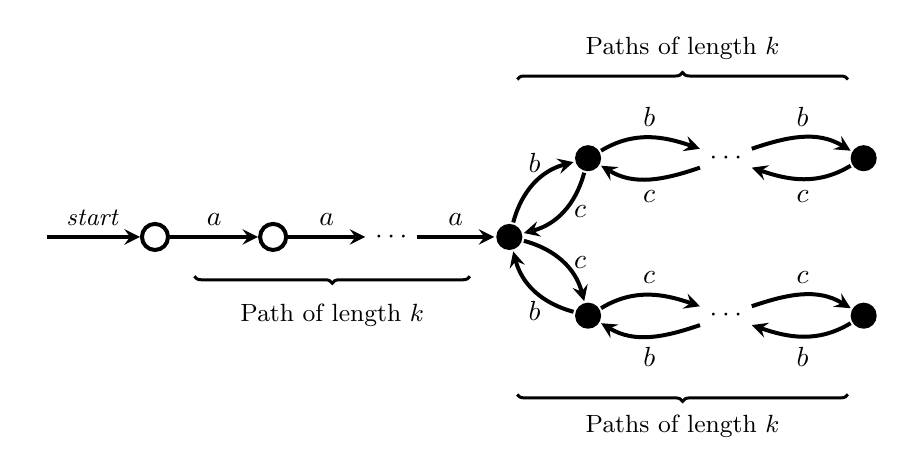
\begin{tikzpicture}
        \node (qs) at (-1.5, 0) {};
        \node[draw, circle, minimum size = 0.1in, line width = 0.02in] (q1) at (0,0) {};
        \node[draw, circle, minimum size = 0.1in, line width = 0.02in] (q2) at (1.5,0) {};
        \node (q3) at (3,0) {$\cdots$};
        \node[fill, circle, minimum size = 0.1in, line width = 0.02in] (qf) at (4.5,0) {};
        \node[fill, circle, minimum size = 0.1in, line width = 0.02in] (b1) at (5.5,1) {};
        \node (b2) at (7.25,1) {$\cdots$};
        \node[fill, circle, minimum size = 0.1in, line width = 0.02in] (b3) at (9,1) {};
        \node[fill, circle, minimum size = 0.1in, line width = 0.02in] (c1) at (5.5,-1) {};
        \node (c2) at (7.25,-1) {$\cdots$};
        \node[fill, circle, minimum size = 0.1in, line width = 0.02in] (c3) at (9,-1) {};

        \draw[-stealth, line width = 0.02in] (qs) -- node[above] {\small\textit{start}} (q1);
        \draw[-stealth, line width = 0.02in] (q1) -- node[above] {$a$} (q2);
        \draw[-stealth, line width = 0.02in] (q2) -- node[above] {$a$} (q3);
        \draw[-stealth, line width = 0.02in] (q3) -- node[above] {$a$} (qf);

        \draw[-stealth, line width = 0.02in] (qf) edge[bend right, out=30, in = 150] node[above] {$b$} (b1);
        \draw[-stealth, line width = 0.02in] (b1) edge[bend right, out=30, in = 150] node[right] {$c$} (qf);
        \draw[-stealth, line width = 0.02in] (b1) edge[bend right, out=30, in = 160] node[above] {$b$} (b2);
        \draw[-stealth, line width = 0.02in] (b2) edge[bend right, out=20, in = 150] node[below] {$c$} (b1);
        \draw[-stealth, line width = 0.02in] (b2) edge[bend right, out=20, in = 150] node[above] {$b$} (b3);
        \draw[-stealth, line width = 0.02in] (b3) edge[bend right, out=30, in = 160] node[below] {$c$} (b2);

        \draw[-stealth, line width = 0.02in] (qf) edge[bend right, out=30, in = 150] node[right] {$c$} (c1);
        \draw[-stealth, line width = 0.02in] (c1) edge[bend right, out=30, in = 150] node[below] {$b$} (qf);
        \draw[-stealth, line width = 0.02in] (c1) edge[bend right, out=30, in = 160] node[above] {$c$} (c2);
        \draw[-stealth, line width = 0.02in] (c2) edge[bend right, out=20, in = 150] node[below] {$b$} (c1);
        \draw[-stealth, line width = 0.02in] (c2) edge[bend right, out=20, in = 150] node[above] {$c$} (c3);
        \draw[-stealth, line width = 0.02in] (c3) edge[bend right, out=30, in = 160] node[below] {$b$} (c2);
        
        \draw[line width = 0.015in, decoration={brace, mirror}, decorate] (0.5, -0.5) -- (4, -0.5);
        \node at (2.25, -1) {\small Path of length $k$};

        \draw[line width = 0.015in, decoration={brace}, decorate] (4.6, 2) -- (8.8, 2);
        \node at (6.7, 2.4) {\small Paths of length $k$};
        \draw[line width = 0.015in, decoration={brace, mirror}, decorate] (4.6, -2) -- (8.8, -2);
        \node at (6.7, -2.4) {\small Paths of length $k$};
    \end{tikzpicture}